\question[10] Observa los dos triángulos congruentes de la Figura \ref{fig:congruencia03}  para responder cada pregunta.

\begin{figure}[H]
    \centering
    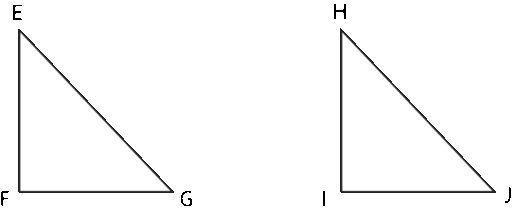
\includegraphics[width=0.45\textwidth]{../images/congruencia03}
    \caption{}
    \label{fig:congruencia03}
\end{figure}
\begin{parts}
    \part El ángulo E es congruente al ángulo \fillin[H][1cm].
    \part $\overline{FG} \cong$  \fillin[$\overline{IJ}$][1cm].
    \part El ángulo J es congruente al ángulo \fillin[G][1cm].

\end{parts}